\chapter{Exploring the neuroprotective effects of tibolone during astrocytic metabolic inflammation: a flux balance analysis approach}
\section*{Abstract:}
\section{Introduction}
\subsection*{Astrocyte-Neuron Metabolic Relationships}
Astrocytes are the most abundant cells in the human brain and play important roles in the central nervous system (CNS) \cite{Takuma2004}. They are highly associated to several homeostatic functions such as glutamate, ion, and water homeostasis, energy storage in the form of glycogen, synapse formation and remodeling, defense against oxidative stress, scar formation, tissue repair and modulation of synaptic activity via the release of gliotransmitters \cite{Lange2012}. Astrocytes metabolize glucose in anaerobic way to produce lactate, which is released to neurons through monocarboxylate transporters \cite{Kimelberg2010}. Lactate is used in neurons as an energy substrate after its convertion to pyruvate and subsequently to ATP via oxidative phosphorylation \cite{Allen2009}. Astrocytes play an important role in glutamate mediated synaptic activity \cite{Halassa2010}; according to the astrocyte–neuron lactate shuttle model, astrocytes respond to glutamate induced activation by increasing their rate of glucose uptake and the release of lactate into the extracellular space, increasing the lactate available to be used by neurons to supply their energetic needs \cite{Giaume2010}. Glutamate is uptaked by astrocytes through the glutamate aspartate transporter and glial glutamate transporter-1, inducing events that involves the activation of Na$^+$–K$^+$-ATPase and maintaining extracellular glutamate at homeostatic levels \cite{Nijboer2013}. Part of incorporated glutamate is converted to glutamine through glutamine synthetase, which is only associated to glial cells and released to neurons using electroneutral systems-N transporters coupled to Na$^+$ and H$^+$ \cite{Barres2008}. In neurons glutaminase enzyme converts glutamine back into glutamate which can be used again for neurotransmission or metabolized into the neuronal Krebs cycle \cite{Shen2013}. Astrocytes release many other substances related to synaptic transmission \cite{Petrelli2016}. However D-serine, a neurotransmitter that act as a coagonist with glutamate at NMDA receptors is one of the most important \cite{Halassa2010}. Due in brain only glial cells can synthesize serine, all available D-serine at synapsis is associated to be primarily produced and secreted by astrocytes \cite{Barres2008}. D-serine is synthesized in astrocytes by serine racemase from L-serine \cite{Durrant2014}. Additionally to these energy and synaptic support associated functions, astrocytes also play an important role in the reduced glutathione (GSH) metabolism of the brain \cite{Raps1989}. GSH is the major cellular antioxidant and plays an important neuroprotective role \cite{Jha2016}. Cellular GSH levels are closely correlated with cell survival under adverse conditions \cite{Allaman2011}. GSH is synthesized from glutamate, cysteine, and glycine and release directly from astrocytes through GSH transporters ion-independent and its net transport is concentration-gradient dependent \cite{Wang2000}. This strong metabolic cooperation between astrocytes and neurons allows to predict that even an small astrocytic dysfunction might cause and/or contribute neurodegenerative processes \cite{Maragakis2006}. Homeostatic astrocyte function is required for neuronal survival after different brain insults, such as inflammation, glucose deprivation, traumatic brain injury and ischemia \cite{Avila-Rodriguez2014,Jha2016}. Astrocytes protect neurons of the most important factors that contribute to neuronal cell death such as glutamate-mediated excitotoxicity leading to disturbances in calcium and sodium intracellular metabolism, mitochondrial dysfuncion, oxidative stress, cytokines and toxins \cite{Takuma2004,Lange2012,Nijboer2013,Hussain2013}.

\subsection*{Astrocytes response to Inflammation}
Inflammation is a complex biological response to injuries, metabolic disorders or infections and its dysregulation induce many complex diseases through astrocytic dysfunction \cite{Masel2010,Yan2013,Jha2016}. In brain, inflammatory response acts as a defense mechanism against any threat to homeostatic state inducing changes in glucose metabolism and release of proinflammatory factors \cite{Allaman2011}. Inflammation responses in CNS are mediated by glial cells that acquire reactive phenotypes to participate in repair mechanisms \cite{Takuma2004,Fitch2008,Jha2016}. Astrocytes, as glial cells are highly sensitive cells to inflammatory mediators, they respond to inflammation through a complex reaction named astrogliosis \cite{Dowell2009a}. During astrogliosis, glial cells generally associated to several beneficial activities in the CNS, also act as a source of inflammatory mediators and as generators of reactive oxidant species (ROS) that have the potential to damage neurons \cite{Molofsk2012}. Astrogliosis is characterized by a low regulation of mitochondrial dynamics that result in mitochondrial failure \cite{Sidoryk-Wegrzynowicz2013}.  Mitochondrial failure induces the deregulation of Ca$^{2+}$ homeostasis and increased ROS generation, both of which are linked to neurotoxicity \cite{Lange2012}. At metabolic level, inflammatory process has been associated to an increase of free saturated fatty acid in comparison with healthy conditions in some brain tissues \cite{Gupta2012}. The increase of free saturated fatty acid induce metabolic inflammation, a response associated with the induction of diverse intracellular stresses, such as mitochondrial oxidative stress, endoplasmic reticulum stress, and autophagy defects \cite{Jha2016}. Lipid excess in metabolic inflammation activates IKK$\beta$ and NF-$\kappa\beta$ signaling pathways, which ultimately impairs leptin and insulin hormonal signaling and further triggers the synthesis and release of increased amounts of ROS and proinflammatory cytokines (TNF-$\alpha$ and IL-6) from glial cells to sustain the neuroinflammatory state \cite{Purkayastha2015}. Enhanced ROS generation by reactive glial cells trigger mitochondria dysfunction in neuron, which induces neuronal apoptosis, the prerequisite for a diverse number of neurodegenerative conditions \cite{K.2006}.

\subsection*{Systems Biology and  Inflammation}
Inflammatory pathways are evolutionarily conserved, complex, redundant and interconnected \cite{Vodovotz2010} . These characteristics difficult each attempt to understand any disease having inflammation at its core using the traditional reductionism-based scientific method and the current regulatory framework \cite{Vodovotz2008}. Traditional methods generally focus on single molecules and genes as the targets of study and potential therapy development, nevertheless mechanistic simulation through a translational systems biology methods allows lead to an understanding of the origin of patterns based in omic data integration in order to facilitate the design of novel therapies \cite{An2011}. Inflammation is a complex system, which is characterized by sensitivity to initial conditions, positive and negative feedback loops, combined robustness and fragility, and emergence of nonintuitive behaviors \cite{Mi2010}. Translational Systems Biology to inflammation is focused on simulated clinical trials, trying to progress toward personalized diagnostics, personalized medicine, and the rational design of drugs \cite{Vodovotz2010}.

\subsection*{Tibolone}
Drugs as steroids compounds are the most potent and effective agents in controlling chronic inflammatory diseases \cite{Laveti2013}. However, steroids prescription is limited due their adverse side effects \cite{Albertazzi1998}. Some steroids synthesized in the nervous system, called ‘neurosteroids’, display beneficial neuroprotective properties, which may be of particular importance in the treatment of diseases where inflammation and neurodegeneration is predominant including age-dependent dementia, stroke, epilepsy, spinal cord injury, Alzheimer’s disease (AD) and Parkinson’s disease (PD) \cite{Wojtal2006}. Neuroprotective actions of molecules that may imitate the neuroprotective actions of esteroids without the perjudicial side effects, such as selective estrogen receptor modulators (SERMs) and selective tissue estrogenic activity regulators (STEARs) have been tested in previous studies \cite{Kloosterboer2001,Sharma2006}. Tibolone is one of these compounds with SERMs and STEARs activities, traditionally used as hormone replacement therapy in post-menopausal women \cite{Timmer2002}. Tibolone has been shown neuroprotective effects in cultured and under ischemia injury rat neurons \cite{Altinoz2009}. Tibolone is a synthetic steroid drug with estrogenic, progestogenic, and weak androgenic actions; is metabolized in three compounds, two major active metabolites, 3$\alpha$-hydroxytibolone and 3$\beta$-hydroxytibolone acting as potent agonists of the estrogen receptor (ER) and its metabolite $\Delta$4tibolone acting as agonists of the progesterone and androgen receptors \cite{Kloosterboer2004}. Tibolone and their metabolites have tissue selective action mechanisms (progestogenic, androgenic and estrogenic) reported in liver, bone, breast and brain according to receptor interaction and activation \cite{Kloosterboer2001}. Nevertheless, actually is not well know the effects of tibolone over glial cells that allows its neuroprotective action \cite{Avila-Rodriguez2014}. Previous studies have shown that 3-hydroxy-metabolites of tibolone exert agonistic actions on human astrocytes through the activation of estrogen receptors, indicating that astrocytes are a target for tibolone \cite{Altinoz2009}.

In this work we simulate the metabolic inflammatory response in healthy mature astrocytes caused by the increase uptake of palmitate, the most common free saturated fatty acid. We model and simulate the metabolic response using a translational system biology approach called Flux Balance Analysis (FBA) described in methods. We focused in identification of changes in metabolic pathways activation, functional products, gliotransmitter release and the neuroprotective effects mediated by tibolone in the inflammated scenario.
\section{Material and Methods}
\subsection*{Tissue Specific Model Construction}
The tissue specific model construction process started with the identification of all enzyme‐coding genes expressed over the mean in at least 50\% of samples for healthy human astrocytes indexed in the GEO database \cite{Edgar2002} as GSE73721 \citep{Zhang2016}. Gene identificators convertion from GeneCards\cite{rebhan1997genecards} to ENTREZ \cite{maglott2005entrez} was performed throught `UniProt.ws' R Package \cite{Carlson2016}. Reactions associated with the identified genes were mapped from the Human Genome Scale  Metabolic Reconstruction RECON 2.04 downloaded from the VMH Lab (https://vmh.uni.lu) \cite{thiele2013community}. The R package `g2f' \cite{G2F} was used to identify and fill the gaps using all no gene associated reactions included in RECON 2.04, as well as to identify and remove all blocked reactions  from the reconstruction. All reactions involved in the conversion of extracellular glutamate, glycine, cysteine and glucose to extracellular glutamine, glycine, serine-D, reduced glutathione, lactate and ATP respectively were added. Exchange reactions were limited to components of the Dulbecco's Modified Eagle Medium (DMEM) as input and gliotransmitters (glutamine, D-serine, ATP, glutamate), reduced glutathione, lactate, glucose, nitric oxide, prostaglandins and leukotrienes as output. Finally, syntax, mass-charge validation and creation of SBML files were carried out through the `minval' R Package \cite{MINVAL}. Reaction limits (upper and lower bounds) were constrained proportional to the mean gene expression reported for genes included in Gene-Protein-Reaction (GPR) \cite{Thiele2010} associated to each reaction in samples of 47 to 63 years old using `exp2flux' R package \cite{EXP2FLUX}. All analysis were done by the `sybil' \cite{Gelius-Dietrich2013} R Package running under R 3.3.1 \cite{RCoreTeam2016}.
\subsection*{Flux Balance Analysis}
Flux Balance Analysis (FBA) is a linear optimization method for simulating metabolism that allows to identify the set of reactions involved in the production of a biological response within a metabolic model \cite{Orth2010}. The metabolic reactions are represented internally as a stoichiometric matrix ($S$), of size $m * n$, where $m$ represents the compounds and $n$ the reactions; the entries in the matrix are the stoichiometric coefficients of the metabolites participating in a reaction \cite{Raman2009}. The flux through all of the reactions in a network is represented by the vector $v$, which has a length of $n$. The concentrations of all metabolites are represented by the vector $x$, with length $m$. The systems of mass balance equations at steady state, $\dfrac{d_{x}}{d_{t}}=0$ or $S * v = 0$. FBA seeks to maximize or minimize an objective function which can be any linear combination fluxes, to obtain a flux for each reaction, indicating how much each reaction contributes to the objective function \cite{Orth2010}. FBA for healthy, inflammated and medicated scenarios was resolved using GLPK 4.60, setting the generic human biomass reaction included in RECON 2.04 and each one of reactions described in table \ref{OF} as objective functions. Models were analyzed by comparing fluxes between scenarios, metabolites production rate and sensitivity analysis.

\begin{table}[h]
\caption{Main metabolic capabilities associated to astrocytes represented as the set of objective functions used to evaluate neuroprotective effects of Tibolone under inflammated scenarios}
\label{OF}
\begin{center}
\begin{tabular}{rm{6.5cm}m{6cm}}
\hline
ID & FORMULA REACTION & DESCRIPTION \\
\hline
\hline
Glu2Gln & 1 glu\_L[e] $\Rightarrow$ 1 gln\_L[e] & Glutamate - Glutamine Cycle \\
Gly2SerD & 1 gly[e] $\Rightarrow$ 1 ser\_D[e] & Glycine to D-serine conversion\\
Glc2Lac & 1 glc\_D[e] $\Rightarrow$ 2 lac\_L[e]& Lactate production from Glucose \\
Glc2ATP & 1 glc\_D[e] $\Rightarrow$ 36 atp[e] & ATP production from Glucose \\
Cys2GTHRD&1 cys\_L[e] + 1 glu\_L[c] + 1 gly[c] $\Rightarrow$ 1 gthrd[e]& Catch of Cysteine to produce reduced Glutathione \\
\hline
\end{tabular}
\end{center}
\end{table} 
\subsection*{Metabolic Scenarios}
To test neuroprotective effects of tibolone during astrocytic metabolic inflammation we define three different metabolic scenarios. A `healthy' scenario, where palmitate uptake rate was freely set by optimizer; an `inflammated' scenario, where uptake rate of palmitate was forced to be stable in the mean of the half maximal inhibitory concentration (IC50) value for all objective functions included in table \ref{OF}. IC50 values were calculated through a robutness analysis performed using uptake of palmitate (`EX\_hdca(e)' in RECON 2.04) as control reaction and a 1000 points in the range from 0 to 1 mMgDW$^{-1}$h$^{-1}$ for each objective function. Uptake value where each objective function reached IC50 was selected and subsequently averaged. Finally, a medicated scenario, defined as an inflammated scenario that include 279 reactions associated with tibolone and estradiol-derivated compounds metabolism. Ten specific reactions described in table \ref{Tibolone} associated to specific Tibolone action mechanism non included in RECON 2.04 were added to medicated scenario.
\begin{table}[h]
\caption{Set of reactions associated to tibolone specific action mechanism in brain reported by Kloosterboer, H. J. (2004) added to medicated scenario model.}
\label{Tibolone}
\begin{center}
%\footnotesize{
\begin{tabular}{rlm{7cm}}
\hline
ID & FORMULA REACTION & DESCRIPTION \\
\hline
\hline
T1 & tibolone[e] $\Leftrightarrow$ & Tibolone exchange reaction\\
T2 & tibolone[e] $\Leftrightarrow$ a3OHtibolone[e] & 3$\alpha$hidroxytibolone interconvertion\\
T3 & tibolone[e] $\Leftrightarrow$ b3OHtibolone[e] & 3$\beta$hidroxytibolone interconvertion \\
T4 & tibolone[e] $\Rightarrow$ d4tibolone[e] & $\Delta$4tibolone isomer formation \\
T5 & b3OHtibolone[e] $\Rightarrow$ d4tibolone[e] &  $\Delta$4tibolone isomer formation from 3$\beta$-hidroxytibolone \\
T6 & a3OHtibolone[e] $\Rightarrow$ estradiol[c] & Estradiol receptor agonist action mechanism of 3$\alpha$-hidroxytibolone\\
T7 & b3OHtibolone[e] $\Rightarrow$ estradiol[c] & Estradiol receptor agonist action mechanism of 3$\beta$-hidroxytibolone\\
T8 & d4tibolone[e] $\Rightarrow$ prgstrn[c] + tststerone[c] & Progesterone and androgen receptor activation by tibolone $\Delta^4$ isomer\\
T9 & a3OHtibolone[e] $\Leftrightarrow$ a3SOtibolone[e] & 3$\alpha$hidroxytibolone interconvertion to sulfated inactive compounds \\
T10 & a3SOtibolone[e] $\Rightarrow$ & Tibolone inactive form in blood \\ 
\hline
\end{tabular}
\end{center}
\end{table} 
\subsection*{Metabolic Changes}
Metabolic changes across metabolic scenarios were measured through two different approximations. Flux differences for each reaction between optimized scenarios were measured using the fold change calculated as described in equation \ref{fC}.
\begin{ceqn}
\begin{align}
\label{fC}
   foldChange = \dfrac{valueModel2-valueModel1}{\left|valueModel1\right|}
\end{align}
\end{ceqn}
Additionally, to obtain a full perspective about inflammation effects in metabolites production, the production of each metabolite was set as objective function in each metabolic scenario and differences were evaluated as well as flux differences.
\subsection*{Proinflammatory, Antiinflammatory and Tibolone Action Mechanism Associated Enzymes}
Identification of enzymes involved in proinflammatory and antiinflammatory responses as well as in the tibolone action mechanism were identified through several sensitivity analysis as follows: Proinflammatory enzymes, are those that catalyze reactions that being knocked out allows an increase of objective function value. Antiinflammatory enzymes, are those associated to reactions that being knocked out reduce even more the objective function value. Tibolone action mechanism associated enzymes are those that catalyze reactions that being knocked out inhibit entirely the metabolic effect of tibolone.
\section{Results}
\subsection*{Tissue Specific Metabolic Model}
Astrocyte tissue-specific metabolism model has a total of X reactions, with X exchange reactions and X transport reactions. Reactions included in astrocytes metabolism model can be classified on the basis of enzymatic activity (E.C. Number), sub-cellular locations (Compartments), and metabolic pathways (Fig. \ref{}). 

Based in the associated enzyme to each reaction X\% of them are catalyzed by an oxidoreductase enzyme, X\% by an enzyme, X\% by a

A large number of the reactions in the model belonged to the class 1 category of enzyme classification i.e., theoxidoreductases (22 \%).These set of enzymes catalyze the oxidation of one chemical species and the simultaneous reduction of the other bytransfer of electrons fromone species to another. The other classes of enzymes in this classification scheme were the transferases (14 \%) followed by lyases (10 \%), hydrolases (4 \%), isomerases (2 \%), and ligases (2 \%). Another 28 \% of the reactions belonged to transport reactions and 16\% to extracellular exchange reactions,which occurred spontaneously in the system (Fig. 1a). The reactions can also be classified on the basis of their
association with genes to understand gene reaction asso- ciations (Fig. 1b). 60\% of the model reactions were gene- associated, out of which 6\% were transport reactions. 
The rest of the reactions were classified as: Non-Gene associ- ated Exchange Reactions (16 \%), Non-Gene associated Intracellular Reactions (2\%) and Non-Gene associated Transport Reactions (22\%). In In the classification shown in Fig. 1c, the cytosolic and
mitochondrial reactions contributed to 54\% of the total reactions in the model. 2\%of the reactions belonged to the mitochondrial intermembrane space model compartment that specifically accounted for oxidative phosphorylation. The transport reactions were categorized according to the membrane to which it is associated. Transports accounted for 30\% of the total reactions: Mitochondrial membrane spanning (11\%), Nuclear membrane spanning (2\%) and Plasma Membrane spanning (17\%). With reference to the metabolic processes, 23\% of the
reactions belonged to fatty acid metabolism inclusive of both biosynthesis and beta oxidation of palmitic acid. The rest of the pathways contributed to 30\% of the total count of which 14\% belonged to Glycolytic, PPP, TCA cycle and Oxidative phosphorylation pathway and 2\% were contributed each by Glycine–Serine Metabolism, Cysteine Metabolism, Methionine Metabolism and Glutamate Metabolism, without taking into account the transport and exchange reactions. Another set of reactions, namely, cytosolic ATPase (ATPS), cytoplasmic malate dehydro- genase (MDH(Cyto)), Phosphoenolpyruvate carboxykinase (GTP) (PEP\_CarbK\_1), mitochondrial pyruvate carboxy- lase (Pyr\_Carbm) which could not be assigned strictly under any particular pathway, were categorized as ‘Others’ which contributed 2\% of reactions to the (Fig. 1d).
\subsection*{Healthy Scenario}
\subsection*{Inflammated Scenario}
\subsection*{Medicated Scenario}
%Neuronal injury releases glutamate as an important neurotransmitter and this may result in the recruitment and entrapment of neurons in the neuroinflammatory process [Kumar12, 13].
%Neuroinflammation can also lead to homeostatic disturbances, such as iron accumulation, within CNS cells. Iron accumulation has been demonstrated in numerous CNS disorders, including MS, AD, and PD, where it has been postulated to promote disease by augmenting microglial proinflammatory activity, altering mitochondrial function, and inducing ROS production [Kumar18].
%a prominent increase in the expression of the intermediate filament glial fibrillary acidic protein (GFAP) and aldehyde dehydrogenase 1 family member L1 (ALDH1L1) [32]
%Similarly, brain astrocyte- derived ROS, MMP-9, and heme oxygenase-1 (HO-1)/carbon monoxide may contribute to neuronal death [79]
%Their study fur- ther
%demonstrates that activated microglia work
%with astrocytes to cause an elevation of extracellular L-Glu in the early stages of neuroinflammation[110].
%\begin{figure}[h]
%\begin{center}
%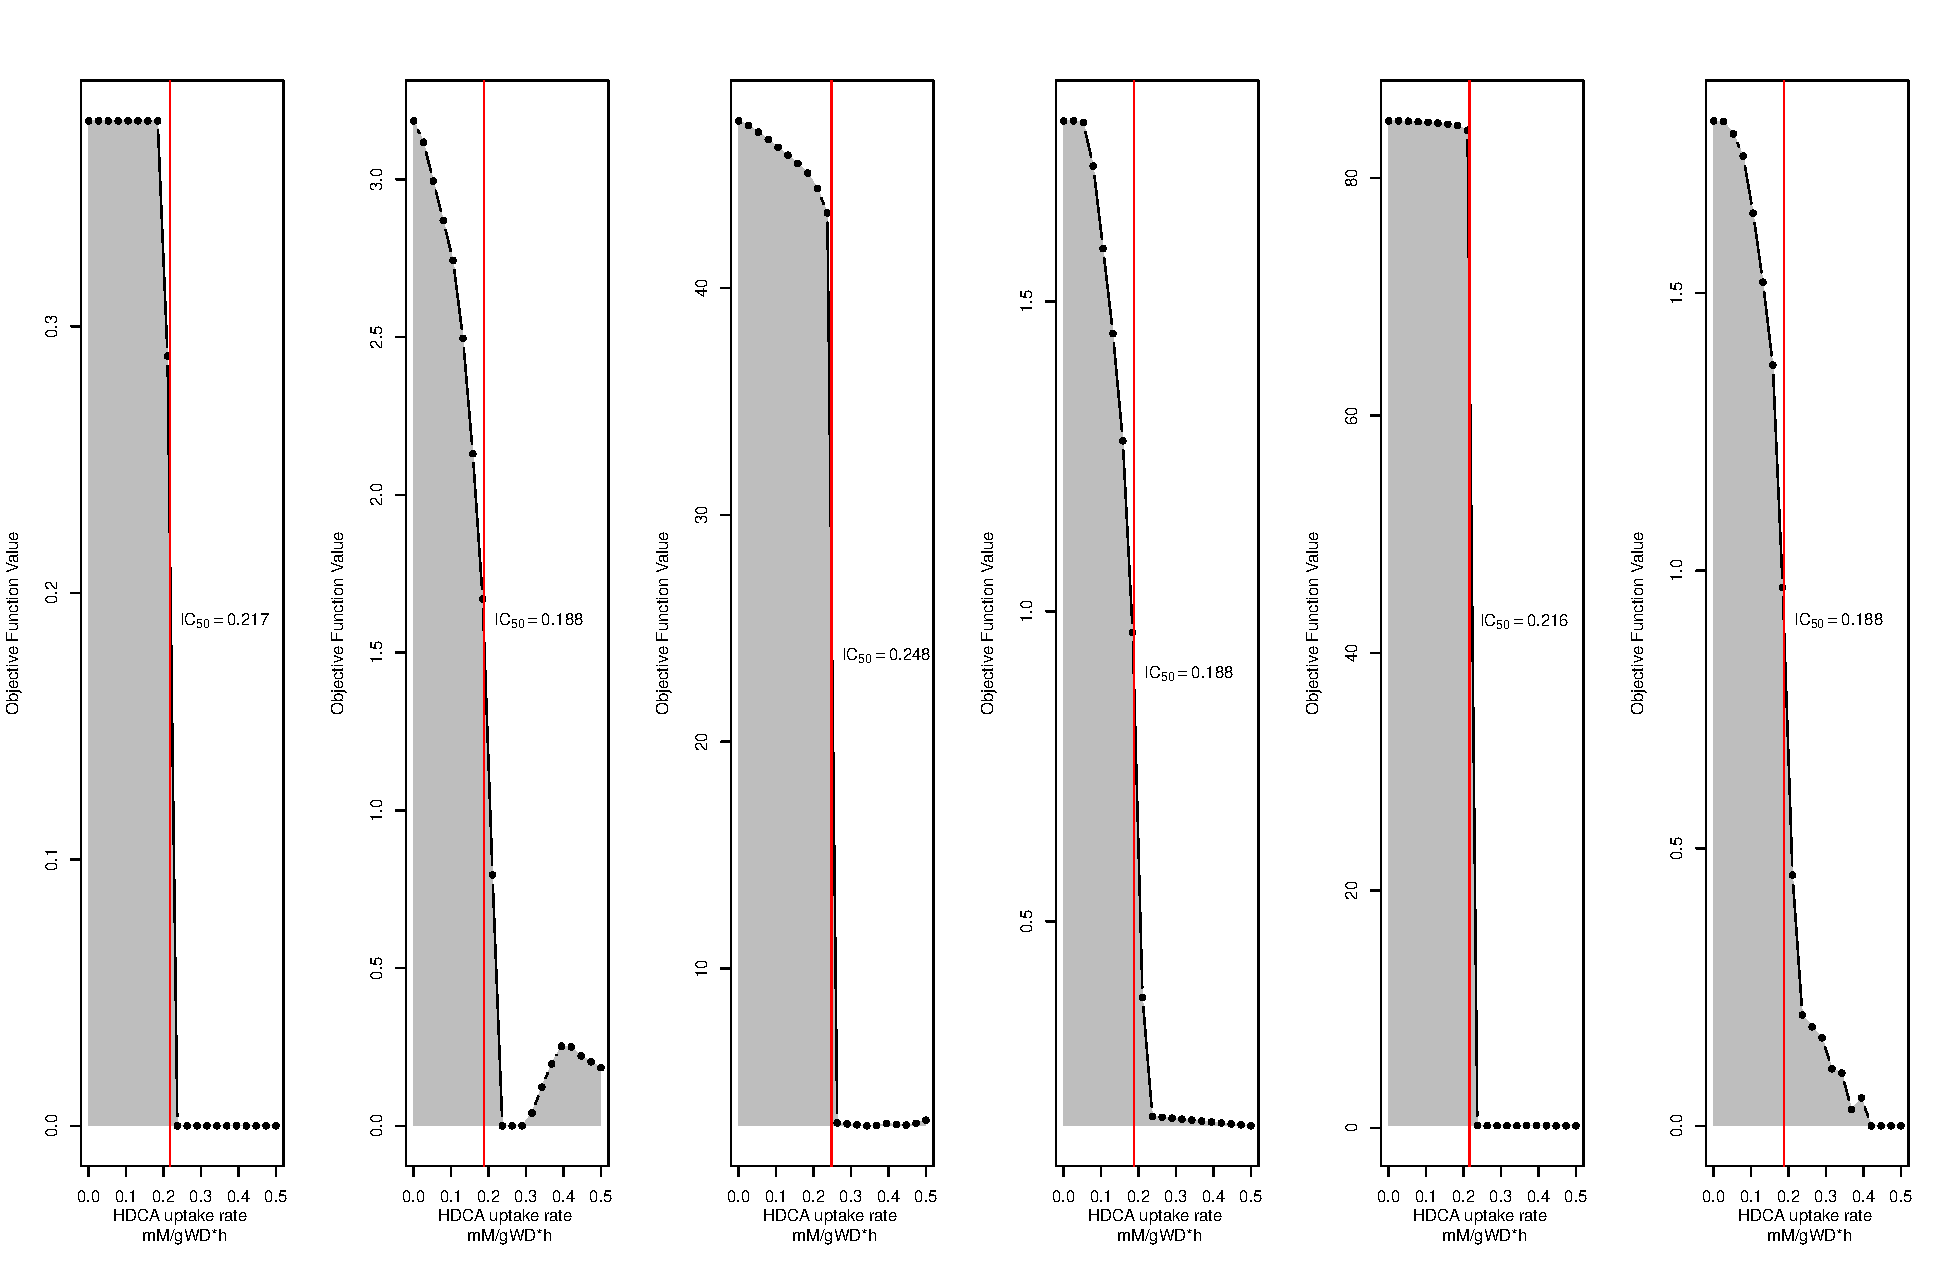
\includegraphics[width=\textwidth]{neuroprotective/IC50}
%\end{center}
%\caption{Robutness analysis to calculate IC50 value for each objective function described in table \ref{OF}. Red line represents the calculated IC50 value.}
%\end{figure}
%\begin{figure}[h]
%\begin{center}
%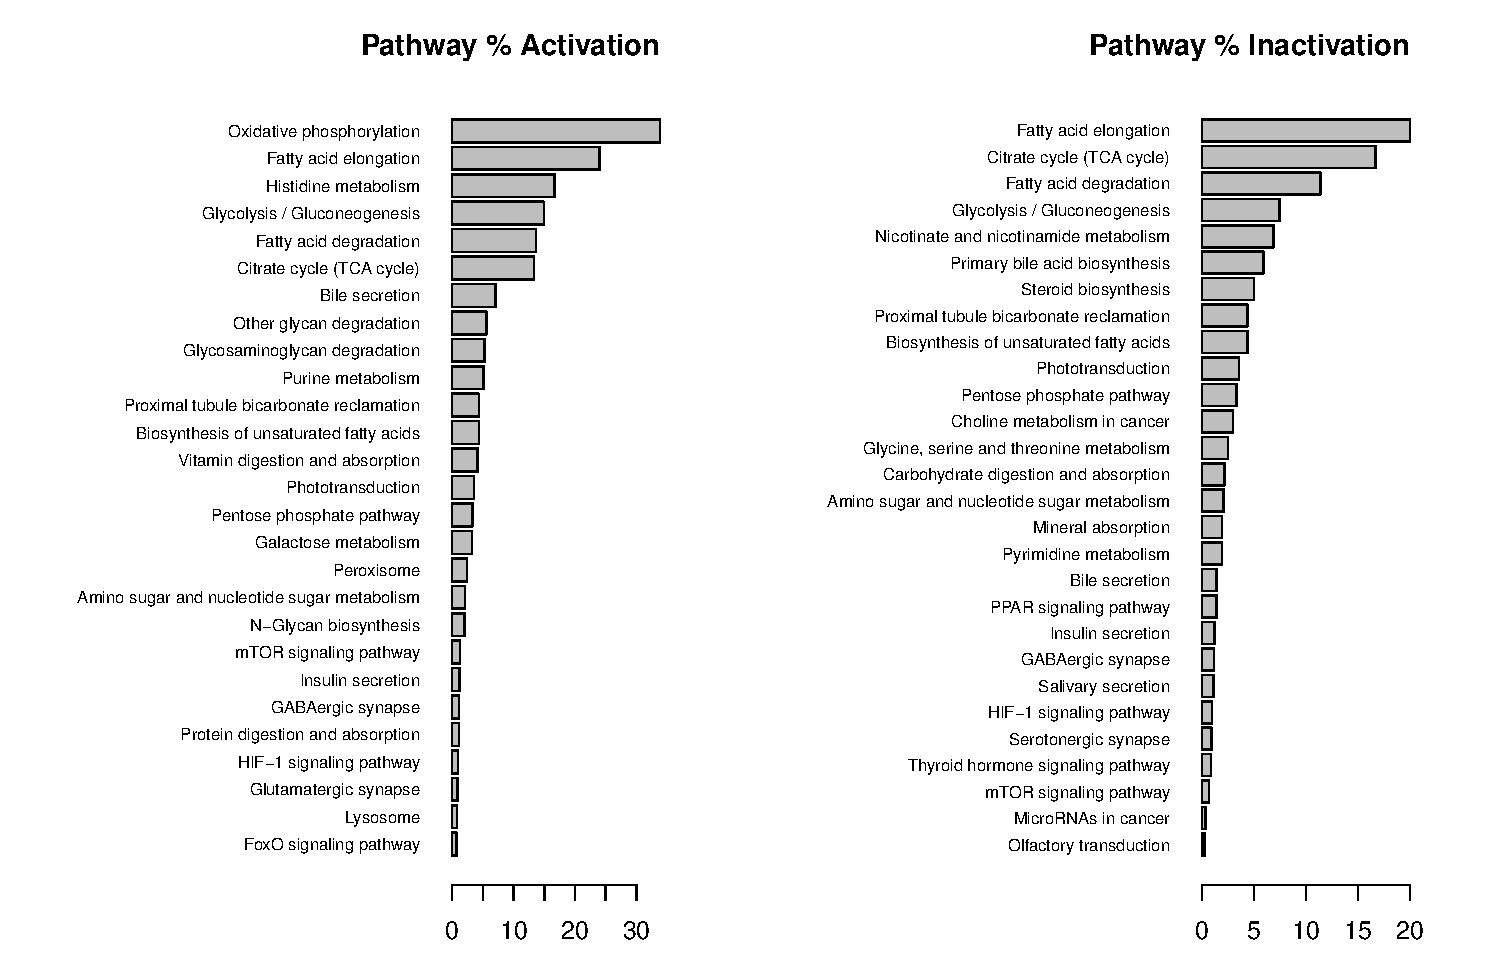
\includegraphics[width=\textwidth]{neuroprotective/Healthy2Inflammated}
%\end{center}
%\caption{Metabolic pathways affected by inflammation. Activation and inactivation percentage was measured in comparison with genes associated to each pathway in the KEGG database.}
%\end{figure}
%\begin{figure}[h]
%\begin{center}
%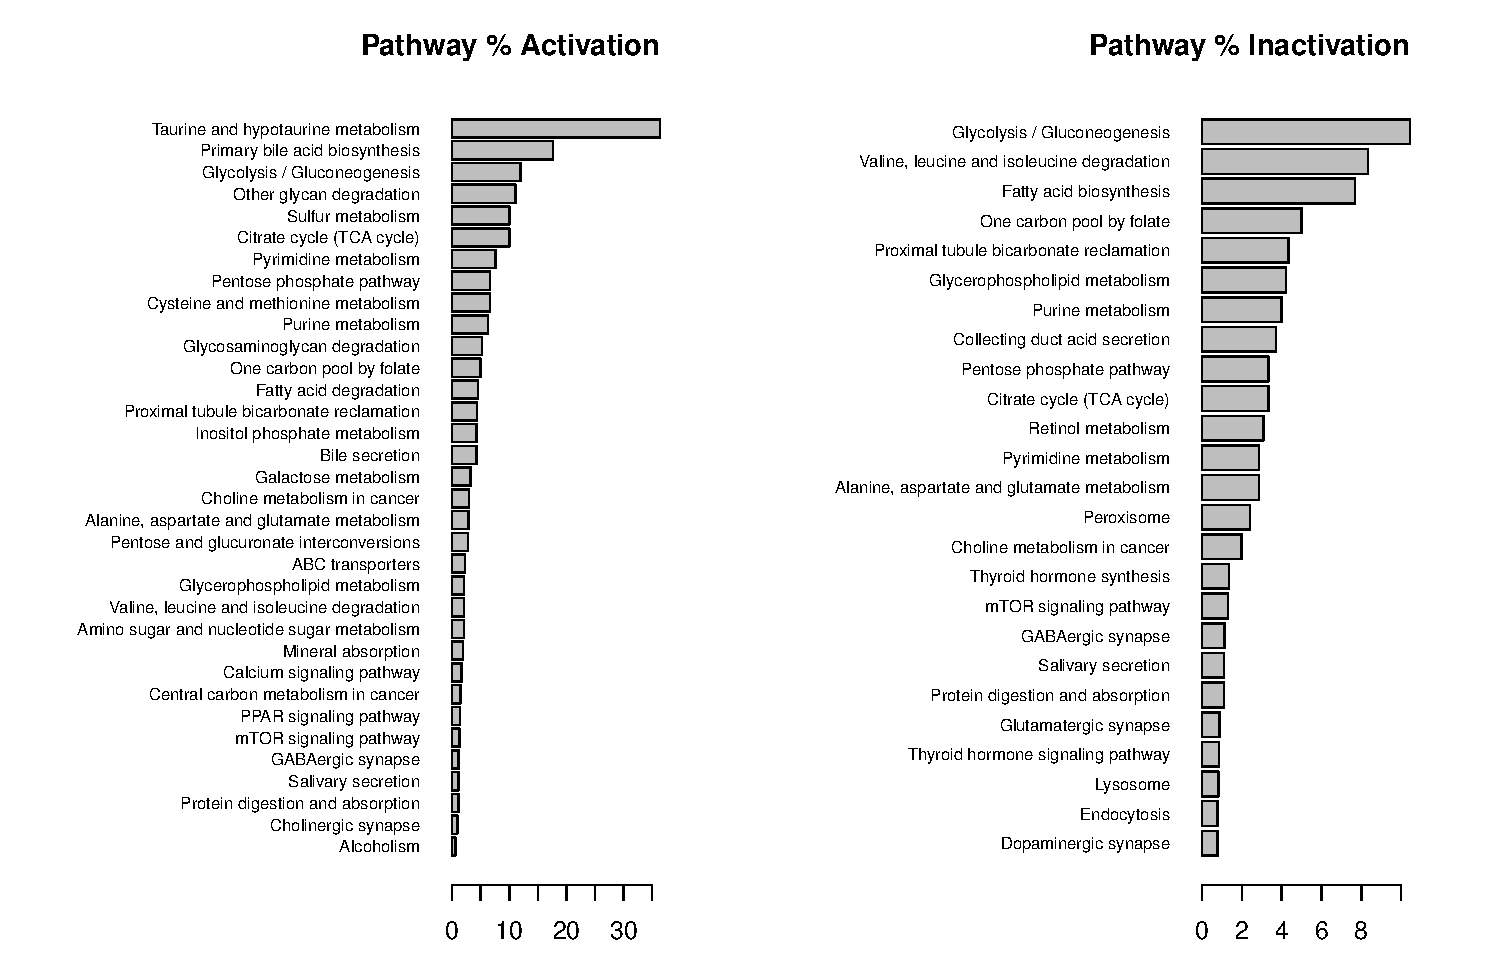
\includegraphics[width=\textwidth]{neuroprotective/Inflammated2Tibolone}
%\end{center}
%\caption{•}
%\end{figure}
\section{Conclusion}
